\section{Finite-size experiments}
\label{sec:main-experiments}

We evaluate four hidden forest families with an exact frozen conditional
oracle at five sizes from $N=8192$ to $16384$.
\textcolor{red}{Figure~\ref{fig:ideal-fixed-accuracy} compares total oracle submissions}
under the fixed empirical batch-KL criterion
$K+2\operatorname{SE}_{\mathrm{MC}}\le10^{-10}L_0$,
\textcolor{red}{where $K$ sums product-to-joint batch KL along the sampled history,
not the target-to-output risk. The family-specific reference $L_0$ is the
one-batch KL cost at $N=2048$ (Appendix~\ref{app:experiments}).
We use empirical tuning; the targets and parameters need not satisfy
the theorem's sufficient conditions.}
\textcolor{red}{Our sampler's submission counts are consistent with sublinear
scaling over the tested finite-size range. These exact-oracle experiments isolate
submission cost; learned-model accuracy and runtime are outside their scope.}

\begin{figure}[H]
 \centering
 % Please use the same frozen data with submission units in the arXiv plot.
 \ifdefined\ArxivVersion
  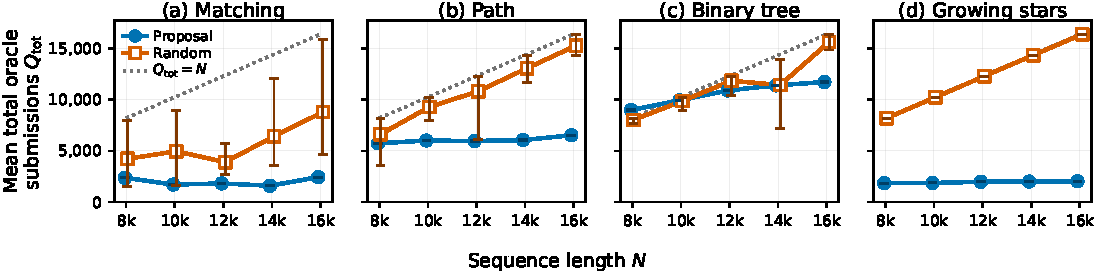
\includegraphics[width=0.88\linewidth]{figures/experiment_submissions_2026-09-27/oracle_submissions.pdf}
 \else
  \includegraphics[width=0.88\linewidth]{../../../experiments/forest_toy/results/ideal_capless_fixed_accuracy_scaling/random_per_run_threshold_search_k1em10L0/ideal_strict_fixed_accuracy_linear_errorbars_1x4_large_text.pdf}
 \fi
 \caption{\textcolor{red}{Total oracle submissions
 $Q_{\mathrm{tot}}=Q_{\mathrm{pre}}+\CounterfactualQueries+\CommitRounds$,
 including preprocessing, probes, and nonempty commit rounds.
 Points: six-run means; whiskers: min--max ranges
 (not standard errors or confidence intervals).
 Proposal settings are fixed per forest and $N$;
 random budgets are selected per run on coupled curves.
 Proposal ranges ($\le78$ submissions) may lie inside markers.
 Dotted line: exact singleton $Q_{\mathrm{tot}}=N$, not a cap.
 Horizontal ticks: $1\mathrm{k}=1024$.}}
 \label{fig:ideal-fixed-accuracy}
\end{figure}
